\section{Temporal stabilization of clusters}

Dopo la clusterizzazione dobbiamo fare un riassegnamento di colori ai clusters per stabilizzarli nel tempo.
Come si è già detto, l'ordine con cui i clusters vengono decisi ad ogni istante è randomico e l'ordine di scelta dei clusters viene rappresentato da un colore. \\
Quindi, dall'iniziale assegnazione di colori randomica, vogliamo passare ad un'assegnazione di colori dove, due clusters dello stesso colore, da un istante all'altro, abbiano in comune più nodi, ossia più joints, possibili. \\
Questo perchè l'assegnazione randomica porta dei problemi a livello di visualizzazione del grafo, in quanto è possibile che da un istante all'altro, due cluster con molte joints in comune abbiano colore diverso e quindi la visualizzazione nel tempo potrebbe risultare come un continuo switch di colori facendo perdere un'idea di continuità.
\\

Per stabilizzare i cluster nel tempo, e quindi far si che le coppie dei vari clusters colorati da un istante all'altro mantengano il maggior numero di joint in comune, ci riconduciamo al Maximum Perfect Weight Matching. \\     
Abbiamo implementato due algoritmi: uno di Brute Force, in cui calcoliamo i pesi totali di tutte le permutazioni degli assegnamenti possibili di colori e scegliamo l'assegnamento con il peso totale massimo, e l'Hungarian Algorithm, un metodo di ottimizzazione combinatoria che risolve in tempo polinomiale il problema dell'assegnamento. \\
Dato che nel nostro caso il numero di cluster è solitamente piccolo, in alcuni casi risulta essere più efficiente l'algoritmo di Brute Force.

\subsection{Maximum Perfect Weight Matching for bipartite graphs}

 Il Maximum Perfect Weight Matching è un problema di ottimizzazione riguardante i grafi. \\
 I grafi in questione sono bipartiti, ossia i vertici possono essere suddivisi in due insiemi distinti in
modo tale che tutti gli archi del grafo connettano vertici di insiemi diversi, ma non ci siano archi che connettano vertici all’interno dello stesso insieme.
Inoltre, questi grafi sono non diretti, ossia la relazione tra due nodi è bidirezionale, in altre parole, l'arco che collega il nodo A al nodo B implica automaticamente l'esistenza dell'arco che collega il nodo B al nodo A. \\
Nel problema del Maximum Perfect Weight Matching i vertici rappresentano gli elementi da accoppiare e gli archi rappresentano le possibili connessioni tra questi elementi. Ogni arco ha associato un peso che rappresenta il valore o l'importanza dell'accoppiamento tra i vertici connessi. \\
 L'obiettivo è trovare un accoppiamento perfetto, ovvero un insieme di archi in cui ogni nodo è connesso esattamente a un altro nodo, senza sovrapposizioni o nodi isolati, massimizzando il peso totale degli archi nell'accoppiamento.
 Il peso totale è la somma dei pesi degli archi inclusi nell'accoppiamento. \\
 I pesi degli archi vengono raccolti in una matrice che prende il nome di matrice di utilità. \\
 La matrice di utilità sarà una matrice quadrata, dato che il numero di nodi facenti parte dei due insiemi distinti è lo stesso.
Le righe potrebbero rappresentare i nodi facenti parte del primo insieme, mentre le colonne potrebbero rappresentare i nodi facenti parte del secondo insieme, oppure viceversa.
 L'elemento (\textit{i}, \textit{j}) della matrice rappresenta il peso dell'arco che collega il vertice \textit{i} al vertice \textit{j}.
 


\subsubsection{Temporal stabilization}
Nel nostro caso, anzichè avere nodi collegati da archi, avremo una situazione leggermente diversa. \\   
Al posto dei nodi introdotti precedentemente, avremo dei clusters, ossia degli insiemi di nodi, che per noi rappresentano le joints dello scheletro, collegati fra loro da archi.
\\  

Consideriamo i clusters all'istante \textit{t} e i clusters all'istante \textit{t+1} come due insiemi distinti, perciò non esisteranno archi che collegano clusters facenti parte dello stesso insieme. \\
Ogni cluster di un insieme deve essere collegato tramite un arco ad uno ed un solo cluster dell'altro insieme, con l'obbiettivo di massimizzare il peso totale degli archi.
Il peso di un arco è pari al numero di nodi che hanno in comune i due clusters che l'arco in questione sta collegando. \\
Come già detto, a questo punto della pipeline, conosciamo già ad ogni istante le joints che fanno parte dei vari clusters e i colori dei vari clusters, ma vogliamo fare un riassegnamento di colori per stabilizzare la visualizzazione nel tempo.
La clusterizzazione precedente raggruppa le varie joints in clusters e gli assegna un colore random, mentre in questa fase della pipeline ottimizziamo l'assegnazione dei colori. \\
Partiremo perciò analizzando i colori dei clusters all'istante iniziale e sceglieremo l'assegnamento migliore di colori per l'istante successivo.
Ripeteremo questo procedimento iterativamente fino all'ultimo istante.


\subsubsection{A real application}
Consideriamo un caso reale per vedere in termini di visualizzazione come funziona il Maximum Perfect Weight Matching. \\
Supponiamo di avere all'istante \textit{t} 20 nodi che rappresentano le joints e 3 clusters labellati di colori diversi, come si può vedere in Figure \ref{fig:clust_t}. \\
All'istante \textit{t+1} ci sono gli stessi 20 nodi precedenti ma 3 clusters labellati differenti (vedi Figure \ref{fig:clust_tplus1}).  \\
Ovviamente questo assegnamento, ottenuto dal clustering, non si può considerare l'assegnamento ottimale, in quanto dobbiamo ancora valutare i \textit{3!} possibili assegnamenti di colore. \\
Conosciamo il colore dei clusters all'istante  \textit{t} e vogliamo assegnare i colori ai clusters all'istante \textit{t+1}.\\
Nella Figure \ref{fig:clust_ass} si possono vedere visivamente tutte i possibili assegnamenti di colore, mentre nella tabella \ref{tab:table_clust} sono raccolti tutti i valori dei nodi comuni per colore e il peso totale del matching.

\begin{figure}[H]
  \centering
  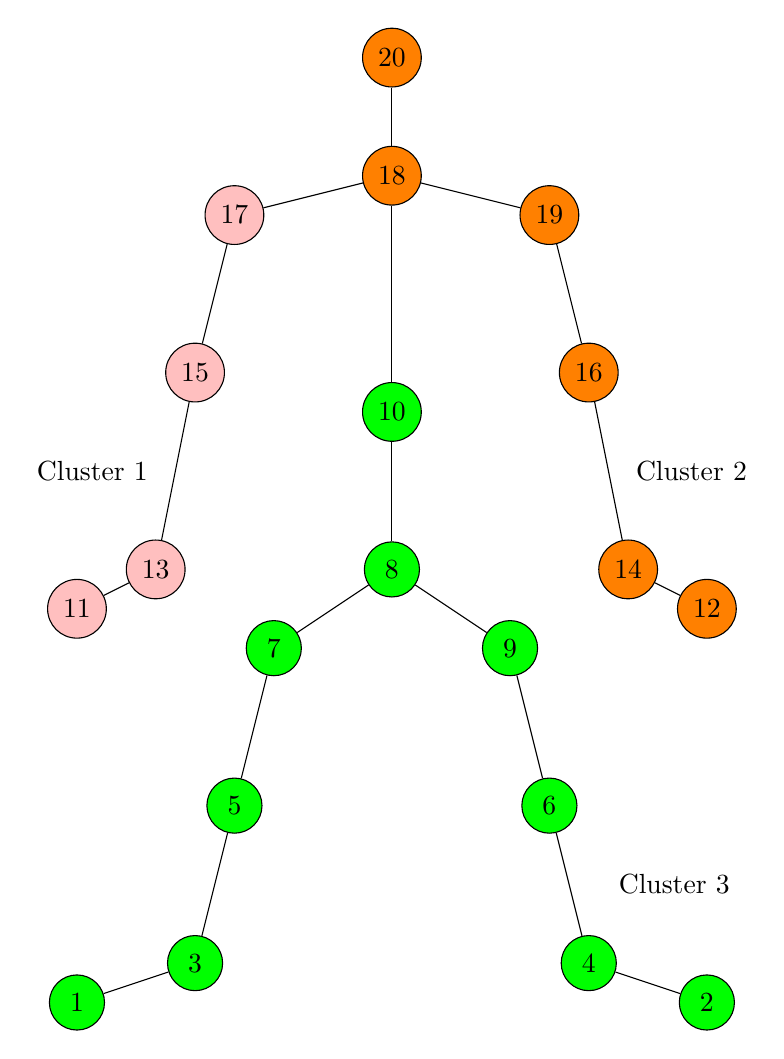
\begin{tikzpicture}
    \node[circle, draw, minimum size=0.7cm] (1) at (1,-9) [fill=green] {1};
    \node[circle, draw, minimum size=0.7cm] (2) at (9, -9) [fill=green] {2};
    \node[circle, draw, minimum size=0.7cm] (3) at (2.5,-8.5) [fill=green] {3};
    \node[circle, draw, minimum size=0.7cm] (4) at (7.5, -8.5) [fill=green] {4};
    \node[circle, draw, minimum size=0.7cm] (5) at (3,-6.5) [fill=green] {5};
    \node[circle, draw, minimum size=0.7cm] (6) at (7,-6.5) [fill=green] {6};
    \node[circle, draw, minimum size=0.7cm] (7) at (3.5,-4.5) [fill=green] {7};
    \node[circle, draw, minimum size=0.7cm] (8) at (5, -3.5) [fill=green] {8};
    \node[circle, draw, minimum size=0.7cm] (9) at (6.5,-4.5) [fill=green] {9};
    \node[circle, draw, minimum size=0.7cm] (10) at (5,-1.5) [fill=green] {10};
    \node[circle, draw, minimum size=0.7cm] (11) at (1,-4) [fill=pink] {11};
    \node[circle, draw, minimum size=0.7cm] (12) at (9,-4) [fill=orange] {12};
    \node[circle, draw, minimum size=0.7cm] (13) at (2, -3.5) [fill=pink] {13};
    \node[circle, draw, minimum size=0.7cm] (14) at (8, -3.5) [fill=orange] {14};
    \node[circle, draw, minimum size=0.7cm] (15) at (2.5,-1) [fill=pink] {15};
    \node[circle, draw, minimum size=0.7cm] (16) at (7.5,-1) [fill=orange] {16};
    \node[circle, draw, minimum size=0.7cm] (17) at (3,1) [fill=pink] {17};
    \node[circle, draw, minimum size=0.7cm] (18) at (5,1.5) [fill=orange] {18};
    \node[circle, draw, minimum size=0.7cm] (19) at (7,1) [fill=orange] {19};
    \node[circle, draw, minimum size=0.7cm] (20) at (5,3) [fill=orange] {20};
    
    \foreach \source/\dest/\label/\xshiftval in {20/18//0, 18/17//0, 18/19//0, 17/15//0, 15/13/Cluster 1/-30, 13/11//0, 19/16//0, 16/14/Cluster 2/30, 14/12//0, 18/10//0, 10/8//0, 8/7//0, 7/5//0, 5/3//0, 3/1//0, 8/9//0, 9/6//0, 6/4/Cluster 3/38, 4/2//0}
      \path (\source) edge node[xshift=\xshiftval] {\label} (\dest);
  \end{tikzpicture}
  \caption{Optimal color assignment to clusters at time \textit{t}}
  \label{fig:clust_t}
\end{figure}


\begin{figure}[H]
    \centering
    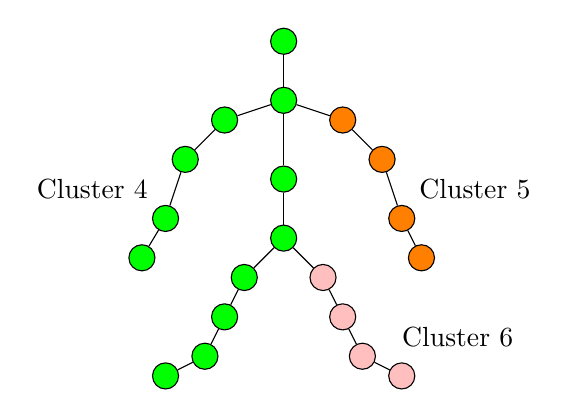
\begin{tikzpicture}
      \node[circle, draw, minimum size=0.1cm] (1) at (3.5,-1.25) [fill=green] {};
      \node[circle, draw, minimum size=0.1cm] (2) at (6.5, -1.25) [fill=pink] {};
      \node[circle, draw, minimum size=0.1cm] (3) at (4,-1) [fill=green] {};
      \node[circle, draw, minimum size=0.1cm] (4) at (6, -1) [fill=pink] {};
      \node[circle, draw, minimum size=0.1cm] (5) at (4.25,-0.5) [fill=green] {};
      \node[circle, draw, minimum size=0.1cm] (6) at (5.75,-0.5) [fill=pink] {};
      \node[circle, draw, minimum size=0.1cm] (7) at (4.5,0) [fill=green] {};
      \node[circle, draw, minimum size=0.1cm] (8) at (5, 0.5) [fill=green] {};
      \node[circle, draw, minimum size=0.1cm] (9) at (5.5,0) [fill=pink] {};
      \node[circle, draw, minimum size=0.1cm] (10) at (5,1.25) [fill=green] {};
      \node[circle, draw, minimum size=0.1cm] (11) at (3.2, 0.25) [fill=green] {};
      \node[circle, draw, minimum size=0.1cm] (12) at (6.75,0.25) [fill=orange] {};
      \node[circle, draw, minimum size=0.1cm] (13) at (3.5, 0.75) [fill=green] {};
      \node[circle, draw, minimum size=0.1cm] (14) at (6.5, 0.75) [fill=orange] {};
      \node[circle, draw, minimum size=0.1cm] (15) at (3.75,1.5) [fill=green] {};
      \node[circle, draw, minimum size=0.1cm] (16) at (6.25,1.5) [fill=orange] {};
      \node[circle, draw, minimum size=0.1cm] (17) at (4.25,2) [fill=green] {};
      \node[circle, draw, minimum size=0.1cm] (18) at (5,2.25) [fill=green] {};
      \node[circle, draw, minimum size=0.1cm] (19) at (5.75,2) [fill=orange] {};
      \node[circle, draw, minimum size=0.1cm] (20) at (5,3) [fill=green] {};  
      \foreach \source/\dest/\label/\xshiftval in {20/18//0, 18/17//0, 18/19//0, 17/15//0, 15/13/Cluster 4/-30, 13/11//0, 19/16//0, 16/14/Cluster 5/30, 14/12//0, 18/10//0, 10/8//0, 8/7//0, 7/5//0, 5/3//0, 3/1//0, 8/9//0, 9/6//0, 6/4/Cluster 6/38, 4/2//0}
        \path (\source) edge node[xshift=\xshiftval] {\label} (\dest);
    \end{tikzpicture}
      \caption{Color assignment to clusters at time \textit{t+1} obtained from clustering}
      \label{fig:clust_tplus1}
\end{figure}


\begin{figure}[H]
  \centering
  \begin{subfigure}{0.45\textwidth}
    \centering
    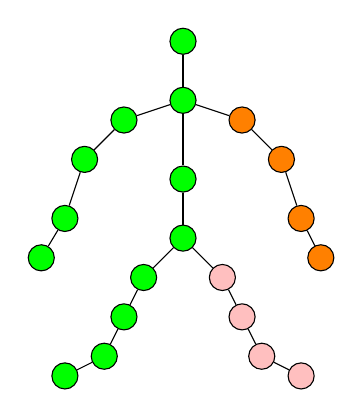
\begin{tikzpicture}[every node/.style={circle, draw, minimum size=0.1cm}]
      \node (1) at (3.5,-1.25) [fill=green] {};
      \node (2) at (6.5, -1.25) [fill=pink] {};
      \node (3) at (4,-1) [fill=green] {};
      \node (4) at (6, -1) [fill=pink] {};
      \node (5) at (4.25,-0.5) [fill=green] {};
      \node (6) at (5.75,-0.5) [fill=pink] {};
      \node (7) at (4.5,0) [fill=green] {};
      \node (8) at (5, 0.5) [fill=green] {};
      \node (9) at (5.5,0) [fill=pink] {};
      \node (10) at (5,1.25) [fill=green] {};
      \node (11) at (3.2, 0.25) [fill=green] {};
      \node (12) at (6.75,0.25) [fill=orange] {};
      \node (13) at (3.5, 0.75) [fill=green] {};
      \node (14) at (6.5, 0.75) [fill=orange] {};
      \node (15) at (3.75,1.5) [fill=green] {};
      \node (16) at (6.25,1.5) [fill=orange] {};
      \node (17) at (4.25,2) [fill=green] {};
      \node (18) at (5,2.25) [fill=green] {};
      \node (19) at (5.75,2) [fill=orange] {};
      \node (20) at (5,3) [fill=green] {};  
      \foreach \source/\dest in {20/18, 18/17, 18/19, 17/15, 15/13, 13/11, 19/16, 16/14, 14/12, 18/10, 10/8, 8/7, 7/5, 5/3, 3/1, 8/9, 9/6, 6/4, 4/2}
        \path (\source) edge (\dest);
    \end{tikzpicture}
      \caption{}
  \end{subfigure}
  \hfill
  \begin{subfigure}{0.45\textwidth}
    \centering
    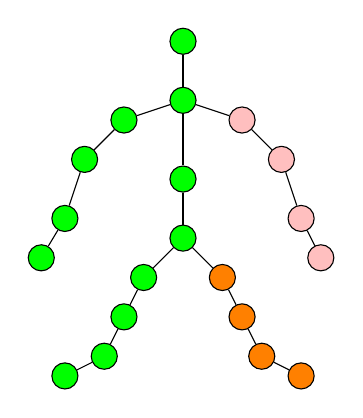
\begin{tikzpicture}[every node/.style={circle, draw, minimum size=0.1cm}]
      \node (1) at (3.5,-1.25) [fill=green] {};
      \node (2) at (6.5, -1.25) [fill=orange] {};
      \node (3) at (4,-1) [fill=green] {};
      \node (4) at (6, -1) [fill=orange] {};
      \node (5) at (4.25,-0.5) [fill=green] {};
      \node (6) at (5.75,-0.5) [fill=orange] {};
      \node (7) at (4.5,0) [fill=green] {};
      \node (8) at (5, 0.5) [fill=green] {};
      \node (9) at (5.5,0) [fill=orange] {};
      \node (10) at (5,1.25) [fill=green] {};
      \node (11) at (3.2, 0.25) [fill=green] {};
      \node (12) at (6.75,0.25) [fill=pink] {};
      \node (13) at (3.5, 0.75) [fill=green] {};
      \node (14) at (6.5, 0.75) [fill=pink] {};
      \node (15) at (3.75,1.5) [fill=green] {};
      \node (16) at (6.25,1.5) [fill=pink] {};
      \node (17) at (4.25,2) [fill=green] {};
      \node (18) at (5,2.25) [fill=green] {};
      \node (19) at (5.75,2) [fill=pink] {};
      \node (20) at (5,3) [fill=green] {};  
      \foreach \source/\dest in {20/18, 18/17, 18/19, 17/15, 15/13, 13/11, 19/16, 16/14, 14/12, 18/10, 10/8, 8/7, 7/5, 5/3, 3/1, 8/9, 9/6, 6/4, 4/2}
        \path (\source) edge (\dest);
    \end{tikzpicture}
      \caption{}
  \end{subfigure}

  \vspace{1cm} % Spazio vuoto tra le righe

  \begin{subfigure}{0.45\textwidth}
    \centering
    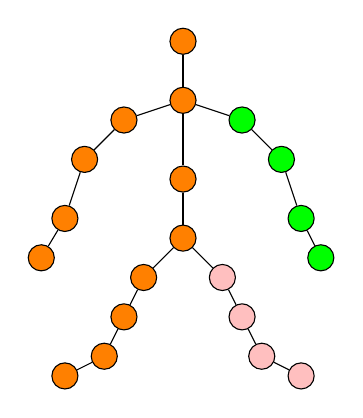
\begin{tikzpicture}[every node/.style={circle, draw, minimum size=0.1cm}]
      \node (1) at (3.5,-1.25) [fill=orange] {};
      \node (2) at (6.5, -1.25) [fill=pink] {};
      \node (3) at (4,-1) [fill=orange] {};
      \node (4) at (6, -1) [fill=pink] {};
      \node (5) at (4.25,-0.5) [fill=orange] {};
      \node (6) at (5.75,-0.5) [fill=pink] {};
      \node (7) at (4.5,0) [fill=orange] {};
      \node (8) at (5, 0.5) [fill=orange] {};
      \node (9) at (5.5,0) [fill=pink] {};
      \node (10) at (5,1.25) [fill=orange] {};
      \node (11) at (3.2, 0.25) [fill=orange] {};
      \node (12) at (6.75,0.25) [fill=green] {};
      \node (13) at (3.5, 0.75) [fill=orange] {};
      \node (14) at (6.5, 0.75) [fill=green] {};
      \node (15) at (3.75,1.5) [fill=orange] {};
      \node (16) at (6.25,1.5) [fill=green] {};
      \node (17) at (4.25,2) [fill=orange] {};
      \node (18) at (5,2.25) [fill=orange] {};
      \node (19) at (5.75,2) [fill=green] {};
      \node (20) at (5,3) [fill=orange] {};  
      \foreach \source/\dest in {20/18, 18/17, 18/19, 17/15, 15/13, 13/11, 19/16, 16/14, 14/12, 18/10, 10/8, 8/7, 7/5, 5/3, 3/1, 8/9, 9/6, 6/4, 4/2}
        \path (\source) edge (\dest);
    \end{tikzpicture}
      \caption{}
  \end{subfigure}
  \hfill
  \begin{subfigure}{0.45\textwidth}
    \centering
    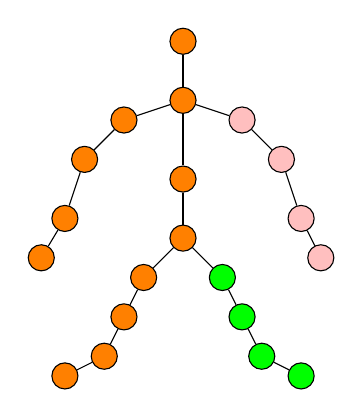
\begin{tikzpicture}[every node/.style={circle, draw, minimum size=0.1cm}]
      \node (1) at (3.5,-1.25) [fill=orange] {};
      \node (2) at (6.5, -1.25) [fill=green] {};
      \node (3) at (4,-1) [fill=orange] {};
      \node (4) at (6, -1) [fill=green] {};
      \node (5) at (4.25,-0.5) [fill=orange] {};
      \node (6) at (5.75,-0.5) [fill=green] {};
      \node (7) at (4.5,0) [fill=orange] {};
      \node (8) at (5, 0.5) [fill=orange] {};
      \node (9) at (5.5,0) [fill=green] {};
      \node (10) at (5,1.25) [fill=orange] {};
      \node (11) at (3.2, 0.25) [fill=orange] {};
      \node (12) at (6.75,0.25) [fill=pink] {};
      \node (13) at (3.5, 0.75) [fill=orange] {};
      \node (14) at (6.5, 0.75) [fill=pink] {};
      \node (15) at (3.75,1.5) [fill=orange] {};
      \node (16) at (6.25,1.5) [fill=pink] {};
      \node (17) at (4.25,2) [fill=orange] {};
      \node (18) at (5,2.25) [fill=orange] {};
      \node (19) at (5.75,2) [fill=pink] {};
      \node (20) at (5,3) [fill=orange] {};  
      \foreach \source/\dest in {20/18, 18/17, 18/19, 17/15, 15/13, 13/11, 19/16, 16/14, 14/12, 18/10, 10/8, 8/7, 7/5, 5/3, 3/1, 8/9, 9/6, 6/4, 4/2}
        \path (\source) edge (\dest);
    \end{tikzpicture}
      \caption{}
  \end{subfigure}
  
  \vspace{1cm} % Spazio vuoto tra le righe


  \begin{subfigure}{0.45\textwidth}
    \centering
    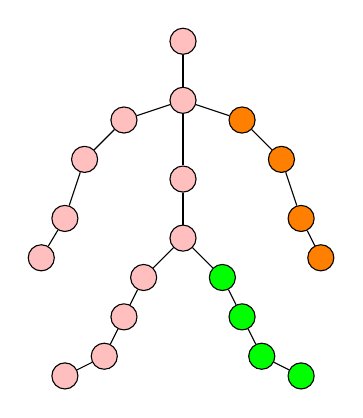
\begin{tikzpicture}[every node/.style={circle, draw, minimum size=0.1cm}]
      \node (1) at (3.5,-1.25) [fill=pink] {};
      \node (2) at (6.5, -1.25) [fill=green] {};
      \node (3) at (4,-1) [fill=pink] {};
      \node (4) at (6, -1) [fill=green] {};
      \node (5) at (4.25,-0.5) [fill=pink] {};
      \node (6) at (5.75,-0.5) [fill=green] {};
      \node (7) at (4.5,0) [fill=pink] {};
      \node (8) at (5, 0.5) [fill=pink] {};
      \node (9) at (5.5,0) [fill=green] {};
      \node (10) at (5,1.25) [fill=pink] {};
      \node (11) at (3.2, 0.25) [fill=pink] {};
      \node (12) at (6.75,0.25) [fill=orange] {};
      \node (13) at (3.5, 0.75) [fill=pink] {};
      \node (14) at (6.5, 0.75) [fill=orange] {};
      \node (15) at (3.75,1.5) [fill=pink] {};
      \node (16) at (6.25,1.5) [fill=orange] {};
      \node (17) at (4.25,2) [fill=pink] {};
      \node (18) at (5,2.25) [fill=pink] {};
      \node (19) at (5.75,2) [fill=orange] {};
      \node (20) at (5,3) [fill=pink] {};  
      \foreach \source/\dest in {20/18, 18/17, 18/19, 17/15, 15/13, 13/11, 19/16, 16/14, 14/12, 18/10, 10/8, 8/7, 7/5, 5/3, 3/1, 8/9, 9/6, 6/4, 4/2}
        \path (\source) edge (\dest);
    \end{tikzpicture}
      \caption{}
  \end{subfigure}
  \hfill
  \begin{subfigure}{0.45\textwidth}
    \centering
    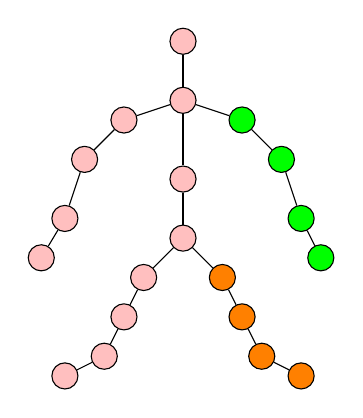
\begin{tikzpicture}[every node/.style={circle, draw, minimum size=0.1cm}]
      \node (1) at (3.5,-1.25) [fill=pink] {};
      \node (2) at (6.5, -1.25) [fill=orange] {};
      \node (3) at (4,-1) [fill=pink] {};
      \node (4) at (6, -1) [fill=orange] {};
      \node (5) at (4.25,-0.5) [fill=pink] {};
      \node (6) at (5.75,-0.5) [fill=orange] {};
      \node (7) at (4.5,0) [fill=pink] {};
      \node (8) at (5, 0.5) [fill=pink] {};
      \node (9) at (5.5,0) [fill=orange] {};
      \node (10) at (5,1.25) [fill=pink] {};
      \node (11) at (3.2, 0.25) [fill=pink] {};
      \node (12) at (6.75,0.25) [fill=green] {};
      \node (13) at (3.5, 0.75) [fill=pink] {};
      \node (14) at (6.5, 0.75) [fill=green] {};
      \node (15) at (3.75,1.5) [fill=pink] {};
      \node (16) at (6.25,1.5) [fill=green] {};
      \node (17) at (4.25,2) [fill=pink] {};
      \node (18) at (5,2.25) [fill=pink] {};
      \node (19) at (5.75,2) [fill=green] {};
      \node (20) at (5,3) [fill=pink] {};  
      \foreach \source/\dest in {20/18, 18/17, 18/19, 17/15, 15/13, 13/11, 19/16, 16/14, 14/12, 18/10, 10/8, 8/7, 7/5, 5/3, 3/1, 8/9, 9/6, 6/4, 4/2}
        \path (\source) edge (\dest);
    \end{tikzpicture}
      \caption{}
  \end{subfigure}
  \caption{Possible color assignments at time \textit{t+1}}
  \label{fig:clust_ass}
\end{figure}



\begin{table}[H]
  \centering
  \begin{tabular}{|c|c|c|c|c|}
    \hline
    Assignment & Pink match & Orange match & Green match & Final cost \\
    \hline
    (a) & 0 & 4 & 6 & 10 \\
    \hline
    (b) & 0 & 0 & 6 & 6 \\
    \hline
    (c) & 0 & 2 & 0 & 2 \\
    \hline
    (d) & 0 & 2 & 0 & 2 \\
    \hline
    (e) & 4 & 4 & 4 & 12 \\
    \hline
    (f) & 4 & 0 & 4 & 8 \\
    \hline
  \end{tabular}
  \caption{Matching weights for the 6 assignments}
  \label{tab:table_clust}
\end{table}
 
Dalla tabella \ref{tab:table_clust} si può notare che l'assegnamento (e) è l'assegnamento con peso più alto.
Inoltre, anche visivamente, si può notare che è l'assegnamento più coerente rispetto a quello dell'istante \textit{t}.
\\

Dal punto di vista del Matching Bipartito, possiamo considerare nella prima partizione i cluster di Figure \ref{fig:clust_t}, mentre nella seconda partizione possiamo considerare i clusters della Figure \ref{fig:clust_tplus1}.
Come già detto, il peso di un arco è equivalente al numero di nodi che hanno in comune quei due clusters che vengono collegati dall'arco in questione. \\
In rosso sono evidenziati gli archi dell'assegnamento (e).


\begin{figure}[H]
  \centering
  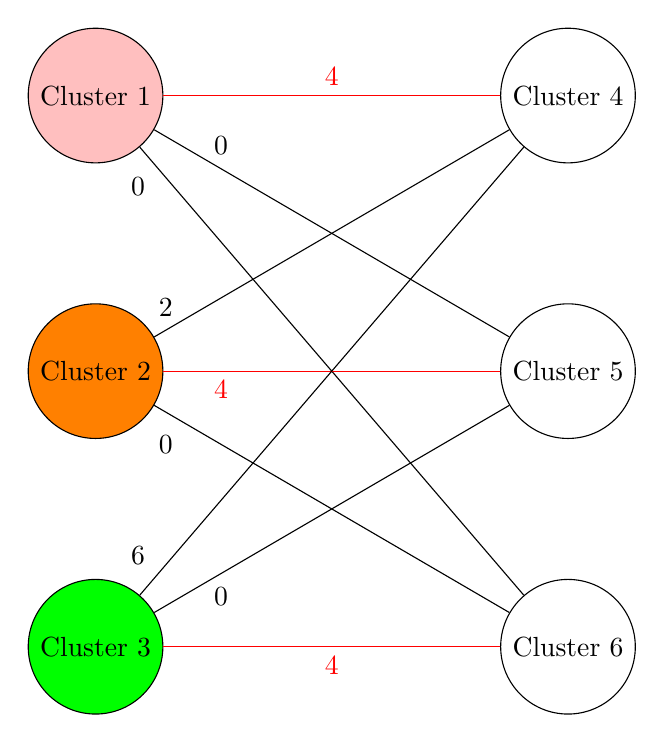
\begin{tikzpicture}
    \node[circle, draw, minimum size=1cm, fill=pink] (1) at (2,-6.5) {Cluster 1};
    \node[circle, draw, minimum size=1cm, fill=orange] (2) at (2, -10) {Cluster 2};
    \node[circle, draw, minimum size=1cm, fill=green] (3) at (2,-13.5) {Cluster 3};
    \node[circle, draw, minimum size=1cm] (4) at (8, -6.5) {Cluster 4};
    \node[circle, draw, minimum size=1cm] (5) at (8,-10) {Cluster 5};
    \node[circle, draw, minimum size=1cm] (6) at (8,-13.5) {Cluster 6};
    
    \foreach \source/\dest/\label/\position/\yshiftval/\xshiftval/\edgecolor in {
      1/4/4/above/0/0/red, 1/5/0/above/25/-40/black, 1/6/0/above/60/-70/black,
      2/4/2/below/-20/-60/black, 2/5/4/below/0/-40/red, 2/6/0/below/30/-60/black,
      3/4/6/below/-60/-70/black, 3/5/0/below/-25/-40/black, 3/6/4/below/0/0/red}
      \path (\source) edge[\edgecolor] node[\position, yshift=\yshiftval, xshift=\xshiftval] {\label} (\dest);
  \end{tikzpicture}
  \caption{Matching from instant \textit{t} to instant \textit{t+1}}
  \label{fig:clust_match}
\end{figure}



\subsection{Brute Force Algorithm}
L'algoritmo di Brute Force può essere una possibile strada per risolvere il problema del MWPM per grafi bipartiti.
Il Brute Force ha una complessità esponenziale, in particolare, la complessità temporale dell'algoritmo cresce in modo esponenziale rispetto al numero di vertici nel grafo.
Questo perché l'algoritmo di Brute Force esamina tutte le possibili combinazioni di abbinamenti perfetti all'interno del grafo bipartito per trovare quello con il peso massimo. \\
Se il grafo ha \textit{n} vertici sia nella prima partizione che nella seconda partizione, ci sono \textit{n}!\ abbinamenti possibili.
Ogni abbinamento richiede \textit{O}(\textit{n}) tempo per essere calcolato, poiché si deve verificare che sia perfetto e quindi calcolare il suo peso totale.
Quindi, la complessità complessiva dell'algoritmo è dell'ordine di \textit{O}(\textit{n}!$\cdot$\textit{n}). \\
Dato che la complessità cresce rapidamente all'aumentare di \textit{n}, diventa rapidamente inattuabile per grafi di grandi dimensioni, ma per il nostro caso questo non è un problema.

A maximum-weight matching problem using an utility matrix can be transformed into a minimum-weight matching problem.
This can be achieved by introducing an auxiliary matrix, referred to as the "cost matrix."
The cost matrix is essentially a duplicate of the utility matrix, but with all its elements negated.

\subsubsection{Brute Force Algorithm summarized}
The operation of the Brute Force algorithm for minimum-weigth matching problems can be summerized in these 3 steps:

\begin{enumerate}
    \item {Compute the cost matrix for the considered bipartite graph with \textit{n} vertoces in each partition.}
    \item {Compute the total cost of all the \textit{n}!\ permutations.}
    \item {Choose the assignment with the lowest total cost.}
\end{enumerate}


\subsubsection{Brute Force Algorithm application}

Let's take for example the following cost matrix and try to apply the Brute Force algorithm for minimum-weigth matching problems:

\begin{table}[H]
    \centering
    \begin{tabular}{|m{0.5cm}|m{0.5cm}|m{0.5cm}|}
      \hline
      108 & 125 & 150 \\
      \hline
      150 & 135 & 175 \\
      \hline
      122 & 148 & 250 \\
      \hline
    \end{tabular}
    \end{table}

Now we compute the total cost of all the \textit{n}!\ permutations: 

\begin{table}[H]
    \begin{minipage}[b]{0.3\textwidth}
      \centering
      \begin{tabular}{|m{0.5cm}|m{0.5cm}|m{0.5cm}|}
        \hline
        \cellcolor{yellow!25} 108 & 125 & 150 \\
        \hline
        150 & \cellcolor{yellow!25} 135 & 175 \\
        \hline
        122 & 148 & \cellcolor{yellow!25} 250 \\
        \hline
      \end{tabular}
      \caption{Total weight: 493}
      \label{tab:perm1}
    \end{minipage}
    \hfill
    \begin{minipage}[b]{0.3\textwidth}
      \centering
      \begin{tabular}{|m{0.5cm}|m{0.5cm}|m{0.5cm}|}
        \hline
        108 & \cellcolor{yellow!25} 125 & 150 \\
        \hline
        150 & 135 & \cellcolor{yellow!25}175 \\
        \hline
        \cellcolor{yellow!25}122 & 148 & 250 \\
        \hline
      \end{tabular}
      \caption{Total weight: 422}
      \label{tab:perm2}
    \end{minipage}
    \hfill
    \begin{minipage}[b]{0.3\textwidth}
      \centering
      \begin{tabular}{|m{0.5cm}|m{0.5cm}|m{0.5cm}|}
        \hline
        108 & 125 & \cellcolor{yellow!25}150 \\
        \hline
        \cellcolor{yellow!25} 150 &  135 & 175 \\
        \hline
        122 & \cellcolor{yellow!25} 148 & 250 \\
        \hline
      \end{tabular}
      \caption{Total weight: 448}
      \label{tab:perm3}
    \end{minipage}
  \end{table}
  

\begin{table}[H]
    \begin{minipage}[b]{0.3\textwidth}
      \centering
      \begin{tabular}{|m{0.5cm}|m{0.5cm}|m{0.5cm}|}
        \hline
        108 & 125 & \cellcolor{yellow!25} 150 \\
        \hline
        150 & \cellcolor{yellow!25} 135 & 175 \\
        \hline
        \cellcolor{yellow!25} 122 & 148 & 250 \\
        \hline
      \end{tabular}
      \caption{Total weight: 407}
      \label{tab:perm4}
    \end{minipage}
    \hfill
    \begin{minipage}[b]{0.3\textwidth}
      \centering
      \begin{tabular}{|m{0.5cm}|m{0.5cm}|m{0.5cm}|}
        \hline
        108 & \cellcolor{yellow!25} 125 & 150 \\
        \hline
        \cellcolor{yellow!25} 150 & 135 & 175 \\
        \hline
        122 & 148 & \cellcolor{yellow!25} 250 \\
        \hline
      \end{tabular}
      \caption{Total weight: 525}
      \label{tab:perm5}
    \end{minipage}
    \hfill
    \begin{minipage}[b]{0.3\textwidth}
      \centering
      \begin{tabular}{|m{0.5cm}|m{0.5cm}|m{0.5cm}|}
        \hline
        \cellcolor{yellow!25} 108 & 125 & 150 \\
        \hline
        150 & 135 & \cellcolor{yellow!25} 175 \\
        \hline
         122 & \cellcolor{yellow!25} 148 & 250 \\
        \hline
      \end{tabular}
      \caption{Total weight: 431}
      \label{tab:perm6}
    \end{minipage}
  \end{table}
   
We find that the minimum total cost is given by the assignment in table \ref{tab:perm4}.  

\subsection{Hungarian Algorithm}

The Hungarian matching algorithm, also called the Kuhn-Munkres algorithm, is a \textit{O}($\textit{n}^3$) algorithm that can be used to find maximum-weight matchings in bipartite graphs with \textit{n} vertices for each partition, which is sometimes called the assignment problem.
A bipartite graph can easily be represented by an utility matrix, where the weights of edges are the entries. \\
Come abbiamo già visto nel Brute Force algorithm, i problemi di maximum-weight perfect matching con la matrice di utilità possono essere trasformati in problemi di minimum-weight perfect matching con la matrice di costo.
Spiegheremo l'Hungarian algorithm applicato ai problemi di minimum-weight matching.
\\

\subsubsection{Hungarian Algorithm summarized}

The operation of the Hungarian algorithm for minimum-weigth matching problems can be summerized in these 6 steps:
\begin{enumerate}
    \item {Compute the cost matrix for the considered bipartite graph with \textit{n} vertices in each partition.}
    \item {Subtract the smallest entry in each row from all the other entries in the row. This will make the smallest entry in the row now equal to 0.}
    \item {Subtract the smallest entry in each column from all the other entries in the column. This will make the smallest entry in the column now equal to 0.}
    \item {Draw lines through the row and columns that have the 0 entries such that the fewest lines possible are drawn.}
    \item {If there are n lines drawn, an optimal assignment of zeros is possible and the algorithm is finished. If the number of lines is less than n, then the optimal number of zeroes is not yet reached. Go to the next step.}
    \item {Find the smallest entry not covered by any line. Subtract this entry from each row that isn’t crossed out, and then add it to each column that is crossed out. Then, go back to Step 3.}
\end{enumerate}

\subsubsection{Hungarian Algorithm application}

Let's take for example the same cost matrix of the Brute Force example and try to apply the Hungarian algorithm for minimum-weigth matching problems:

\begin{table}[H]
\centering
\begin{tabular}{|m{0.5cm}|m{0.5cm}|m{0.5cm}|}
  \hline
  108 & 125 & 150 \\
  \hline
  150 & 135 & 175 \\
  \hline
  122 & 148 & 250 \\
  \hline
\end{tabular}
\end{table}

Subtract the smallest value in each row from the other values in the row:

\begin{table}[H]
\centering
\begin{tabular}{|m{0.5cm}|m{0.5cm}|m{0.5cm}|}
  \hline
  0 & 17 & 42 \\
  \hline
  15 & 0 & 40 \\
  \hline
  0 & 26 & 128 \\
  \hline
\end{tabular}
\end{table}

Now, subtract the smallest value in each column from all other values in the column:

\begin{table}[H]
\centering
\begin{tabular}{|m{0.5cm}|m{0.5cm}|m{0.5cm}|}
  \hline
  0 & 17 & 2 \\
  \hline
  15 & 0 & 0 \\
  \hline
  0 & 26 & 88 \\
  \hline
\end{tabular}
\end{table}

There are 2 lines drawn, and 2 is less than 3, so there is not yet the optimal number of zeroes.

\begin{table}[H]
\centering
\begin{tabular}{|m{0.5cm}|m{0.5cm}|m{0.5cm}|}
  \hline
  \cellcolor{gray!25} 0 & 17 & 2 \\
  \hline
  \cellcolor{gray!25} 15 & \cellcolor{gray!25} 0 & \cellcolor{gray!25} 0 \\
  \hline
  \cellcolor{gray!25} 0 & 26 & 88 \\
  \hline
\end{tabular}
\end{table}

Find the smallest entry not covered by any line. Subtract this entry from each row that isn’t crossed out, and then add it to each column that is crossed out. Then, go back to Step 3.
2 is the smallest entry.
First, subtract from the uncovered rows:

\begin{table}[H]
\centering
\begin{tabular}{|m{0.5cm}|m{0.5cm}|m{0.5cm}|}
  \hline
  \cellcolor{gray!25} -2 & 15 & 0 \\
  \hline
  \cellcolor{gray!25} 15 & \cellcolor{gray!25} 0 & \cellcolor{gray!25} 0 \\
  \hline
  \cellcolor{gray!25} -2 & 24 & 86 \\
  \hline
\end{tabular}
\end{table}

Now add to the covered columns:

\begin{table}[H]
\centering
\begin{tabular}{|m{0.5cm}|m{0.5cm}|m{0.5cm}|}
  \hline
  \cellcolor{gray!25} 0 & 15 & 0 \\
  \hline
  \cellcolor{gray!25} 17 & \cellcolor{gray!25} 0 & \cellcolor{gray!25} 0 \\
  \hline
  \cellcolor{gray!25} 0 & 24 & 86 \\
  \hline
\end{tabular}
\end{table}

Now go back to step 3, drawing lines through the rows and columns that have 0 entries:

\begin{table}[H]
\centering
\begin{tabular}{|m{0.5cm}|m{0.5cm}|m{0.5cm}|}
  \hline
  \cellcolor{gray!25} 0 & \cellcolor{gray!25} 15 & \cellcolor{gray!25} 0 \\
  \hline
  \cellcolor{gray!25} 17 & \cellcolor{gray!25} 0 & \cellcolor{gray!25} 0 \\
  \hline
  \cellcolor{gray!25} 0 & 24 & 86 \\
  \hline
\end{tabular}
\end{table}

There are 3 lines (which is nn), so we are done. The assignment will be where the 0's are in the matrix such that only one 0 per row and column is part of the assignment.

\begin{table}[H]
\centering
\begin{tabular}{|m{0.5cm}|m{0.5cm}|m{0.5cm}|}
  \hline
  0 & 15 & \cellcolor{yellow!25} 0 \\
  \hline
  17 & \cellcolor{yellow!25} 0 & 0 \\
  \hline
  \cellcolor{yellow!25} 0 & 24 & 86 \\
  \hline
\end{tabular}
\end{table}

Replace the original values:

\begin{table}[H]
\centering
\begin{tabular}{|m{0.5cm}|m{0.5cm}|m{0.5cm}|}
  \hline
  108 & 125 & \cellcolor{yellow!25} 150 \\
  \hline
  150 & \cellcolor{yellow!25} 135 & 175 \\
  \hline
  \cellcolor{yellow!25} 122 & 148 & 250 \\
  \hline
\end{tabular}
\end{table}

We find that the minimum total cost is given by this assignment.